\section{Grundlagen/VDI-Racer %und Motivation der Arbeit
}
\label{sec:grundlagen}

VDI-Racer ist die interne Bezeichnung für das verwendete Modellfahrzeug. Dieses Fahrzeug soll technisch die Anforderungen erfüllen, an der Autonomous Driving Challenge\footnote{\url{https://www.vdi-adc.de/}} des VDI teil zu nehmen. Als Grundlage dient das MXcarkit (\cite{MXcarkitSpec}) der Firma Mdynamics\footnote{\url{https://mdynamix.de/en/about-us/}}.

\subsection{Stand der Technik}
Das Fahrzeug, sowie Teile der Software sind zu beginn dieses Projektes bereits vorhanden. In dem folgenden Abschnitt wird diese vorhandene Basis näher beleuchtet.

Der technische Stand hat sich im laufe des Projektes mehrmals geändert, ursprünglich war ROS melodic\footnote{\url{http://wiki.ros.org/Distributions}} (ROS 1) als Basis für das Projekt vorhanden. Darauf werden die meisten Tests, die in dieser Arbeit beschrieben sind, ausgeführt.

Aufgrund von Hardware-Änderungen und diversen anderen Projekten an diesem Fahrzeug, wurde das Fahrzeug später auf ROS2 galactic\footnote{\url{https://docs.ros.org/en/galactic/index.html}} migriert. Für das Projekt haben sich dadurch nur geringfügige Einflüsse ergeben, weshalb auf die neuere Struktur nicht näher eingegangen wird.


\begin{description}
    \item [Stand beginn des Projektes] --
    Zu beginn war das Fahrzeug bereits fahrtüchtig. Es war manuell steuerbar und es gab bereits die ersten Versuche einer autonomen Steuerung. Es war jedoch ein anderen Konzept umgesetzt. Ziel war es in diesem Konzept, dass Fahrzeug automatisch durch einen Raum navigieren zu lassen. Dazu sollte über den LIDAR eine Karte erstellt werden, in der sich das Fahrzeug über Anweisungen bewegen kann. Mit dem LIDAR konnte die eigene Position im Raum ermittelt werden und über einfache Befehle war es dann möglich an eine gegebene Stelle zu navigieren. 

    \item [Motivation] --
    Durch den bevorstehenden Wettbewerb des VDI hat sich das Konzept jedoch geändert. 
    Sollte das Fahrzeug sich vorher noch autark durch einen Raum bewegen, soll es nun dazu in der Lage sein verschiedene Disziplinen des VDI-Wettbewerbs zu meistern. 
    
    \item [Wettbewerb] --
    Der VDI-Wettbewerb ist in mehreren Disziplinen unterteilt, die durch ein Regelwerk definiert werden. 
    Eine dieser Disziplinen ist der Time Trial. 
    Ziel ist es in dieser Disziplin, dass das Fahrzeug auf einer Strecke, die durch Markierungen auf dem Boden abgegrenzt ist, möglichst viele Runden innerhalb der Zeit absolviert.\citep[11]{VDI-adc-Regelwerk} Dazu darf das Fahrzeug nicht ferngesteuert sein. 
    Eine Ausnahme dazu stellt der Startbefehl dar. Das Fahrzeug soll jegliche Entscheidungen ob zum Beispiel eine Gerade, eine Linkskurve oder eine Rechtskurve gefahren wird, selbständig treffen und danach handeln. Das Erfolgreiche absolvieren des Time Trails ist die größte treibende Kraft in diesem Projekt.
    
    Das Regelwerk differenziert für den Wettbewerb zwei Kategorien, den \textbf{VDI-Cup} und den \textbf{VDI-SuperCup} \citep[5]{VDI-adc-Regelwerk}. Beim \textbf{VDI Cup} ist die Hardware vorgegeben. Ausschließlich Softwarelösungen beeinflussen hier das Ergebnis. Die Hardware ist bei allen Fahrzeugen gleich oder gleichwertig. Der \textbf{VDI-Supercup} lässt bei der Hardware mehr Freiheitsgrade, hierbei ist es möglich, verschiedene Hardwarelösungen auszuprobieren um eventuell bessere, kostengünstigere oder einfach alternative Lösungen zu entwickeln.
\end{description}%

Prinzipiell ist es möglich mit dem Fahrzeug am VDI-Cup teil zu nehmen, da die Hardware von Mdynamics eigens für den Wettbewerb konzipiert wurde. Durch Anpassungen an der Hardware aus vorangegangenen Projekten und die Verwendung des Lidars wird 2022 vorerst der VDI-Supercup angestrebt. Für kommende Jahre soll der Fokus jedoch auf dem VDI-Cup liegen.

\bigskip 

%%%%%
\subsection{Aufbau / Komponenten des VDI-Racer}
\label{sec:VDI-Racer-Aufbau}

Das Fahrzeug besteht aus verschiedensten Aktoren und Sensoren. Diese Komponenten zusammen bilden das Grundgerüst für die gesamte Arbeit und besteht aus:

\begin{itemize}
    \item Chassis \& Karosserie
    \item Lenkung \& Servomotor
    \item Antrieb \& Motorsteuerung
    \item Stromversorgung Motor 2x LiPo Polymer Akkus 5200mAh 7,4V
    \item Fernsteuerung
    \item Jetson Xavier NX Developer kit (Computereinheit)
    \item Stromversorgung Jetson Powerbank
\end{itemize}

Die Sensorik des Fahrzeugs besteht aus:
\begin{description}
    \item [Inertial Measurement Unit MPU6050] (IMU) ist ein 6-Achsen Sensor-Modul. Aufgeteilt sind diese Achsen in 3-Achsen Beschleunigungssensor und 3-Achsen Gyroskop. Die Einheit kann durch die Fusion dieser Sensoren eine ROS-Sensormessage\footnote{\url{http://docs.ros.org/en/melodic/api/sensor_msgs/html/msg/Imu.html}} erstellen in der die Orientierung, die lineare Beschleunigung und die angulare Beschleunigung enthalten sind. Zudem besitzt die \strong{MPU6050} über eine Temperatursensor.

    \item [LIDAR] ist ein Laser-Sensor der sich um seine Achse rotiert und dabei den Abstand misst. Das Ergebnis ist eine 2D-Abstandsmessung um das Fahrzeug herum.
    
    \item [Kamera] 
    
    \item [Ultraschall-Sensoren] sind in der Lage, Objekte berührungslos zu erkennen und ihre Entfernung zum Sensor zu messen. Die Sensoren sind zwar mit dem MX-carkit mitgeliefert, jedoch noch nicht verbaut. Sie sollen später bei Disziplinen wie das Einparken helfen den Abstand zu Hindernissen zu messen.
    
    \item [Motorwinkel / Radwinkel / Drehzahl] werden von der Motorsteuerung genutzt um die Odometrie des Fahrzeugs zu bestimmen.
\end{description}
\cite{MXcarkitSpec}

\begin{figure}
  \begin{center}
  
    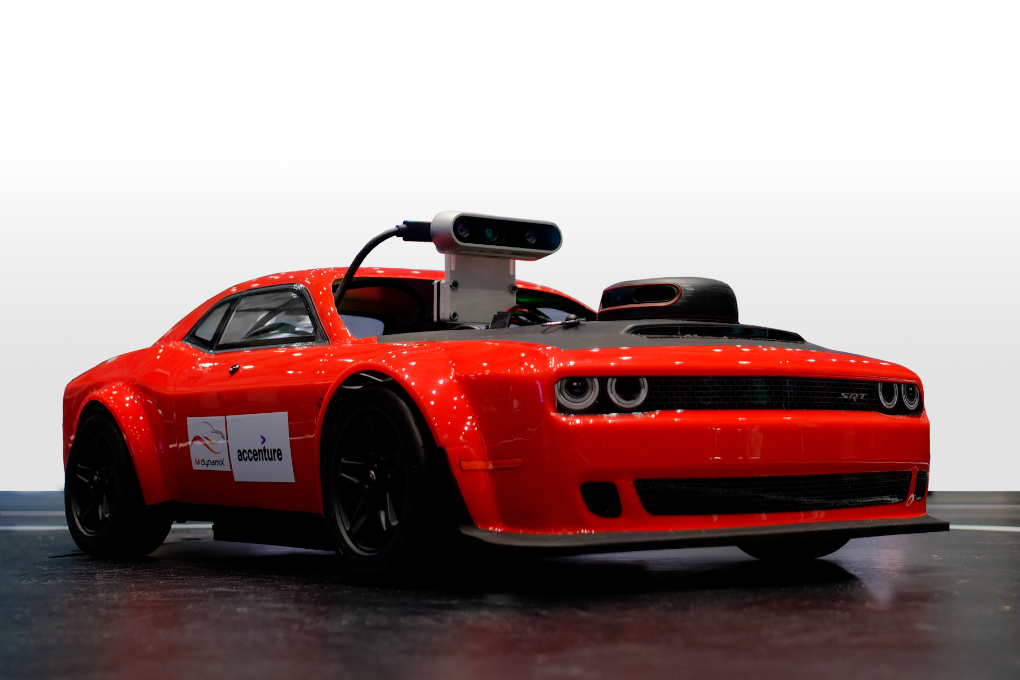
\includegraphics[width=\textwidth]{bilder/VDI-Racer.png}
  \caption{Bild des Fahrzeugs}
  \label{fig:vehicle}
  \end{center}
\end{figure}

\subsection{Grundlagen ROS}
\label{sec:grundlagen-ROS}
Die Software lief ursprünglich auf einem Jetson Xavier NX Computer mit einer ubuntu 18.04 Distribution von NVIDIA. NVDIIA stellt dazu das Jetpack bereit \footnote{\url{https://developer.nvidia.com/embedded/jetpack}}. Zwischenzeitlich hat sich das System geändert und mittlerweile läuft auf dem Computer die ubuntu 20.04LTS Distribution. 

Als Grundlage für die Software wird das Robot Operating System (ROS) verwendet. Dieses bietet schon viele Funktionalitäten und Schnittstellen um einen Roboter oder so wie hier ein Fahrzeug zu automatisieren. Dazu liefert das Framework ein Topic-Publisher/Subscriber-System, dieses ermöglicht einen Datenaustausch zwischen Programmen die sich untereinander nicht kennen müssen. Sie müssen sich nur bei ROS anmelden. Bevor die Programme Nachrichten nutzen können, müssen sie sich lediglich auf eine Syntax der Nachricht geeinigt haben. Dazu bietet ROS schon vordefinierte Nachrichten an, wie zum Beispiel float32\footnote{\url{http://docs.ros.org/en/lunar/api/std_msgs/html/msg/Float32.html}}. 

In der Dokumentation von ROS auf der Wiki-Seite heißt es ``ROS is an open-source, meta-operating system for your robot. It provides the services you would expect from an operating system, including hardware abstraction, low-level device control, implementation of commonly-used functionality, message-passing between processes, and package management. It also provides tools and libraries for obtaining, building, writing, and running code across multiple computers.''
\cite{ROS-Wiki}

\subsection{ ROS-Pakete }
\label{sec:ROS-Pakete}
ROS teilt die einzelnen Module und Funktionalitäten in Pakete auf. Jedes Paket soll dabei eine Aufgabe übernehmen wie zum Beispiel das ansteuern der Motorsteuerung. Diese Informationen werden dann über Topics mit einander getauscht. 
Einige dieser Pakete waren schon vor Beginn des Projektes lauffähig, da Sie in vorangegangenen Projekten erstellt oder eingebunden wurden und bieten einige Funktionalitäten. 

\begin{description}
    \item [vesc] 
    -- Hier steckt die \strong{Motorsteuerung} drin. Dieses Paket erlaubt es, Information an die Motorsteuerung zu senden und zu empfangen. Zudem bietet das Paket mehrere kleinere Nodes, wie zum Beispiel die Übersetzung eines Ackermann-Befehls\footnote{Als AckermannDrive wird im Englischen die Achsschenkellenkung bezeichnet. Der Ackermann-Befehl besteht aus einem Lenk-Winkel, der Geschwindigkeit und noch weiteren Werten. \url{http://docs.ros.org/en/jade/api/ackermann_msgs/html/msg/AckermannDrive.html}} in einen Lenkwinkel für den Servo. Auch die Odometrie wird von diesem Paket geliefert und kann als Topic subscribed werden.
    \item [rc-receiver] 
    -- Das RC-Receiver Paket liefert die Daten der \strong{Fernsteuerung} als Topic. Hierdurch kann das Fahrzeug manuell gesteuert werden. Zudem kann die Fernsteuerung verwendet werden, um einen Modus um zu schalten. 
    \item [mpu6050serial\_to\_imu] 
    \label{item:mpu6050}
    -- Dieses Paket bietet einen Node der den Arduino, an dem eine \strong{IMU} des Typs MPU6050 verbaut ist, ausließt. Zudem erstellt er aus den Daten zwei Topics die von anderen Nodes abgehört (Subscribed) werden können. Einmal die Positions- und Rotationsdaten selbst und die Temperatur werden versendet.
    \item [rplidar] 
    -- Das LIDAR Paket für ROS ist ebenfalls bereits erstellt und liefert eine Punktewolke über einen Topic. Das LIDAR kann den umgebenden Raum in einer 2-Dimensionalen Ansicht darstellen. Zusammen mit anderen Positionsermittelnden Sensoren wie der IMU und der Odometrie kann so die Position im Raum gefunden werden solange eine Karte verfügbar ist.
    %Zusammen mit einer Einschränkung des Winkels wurde dieses Modul lediglich dazu verwendet, den Abstand zu einem Hindernis vor dem Fahrzeug zu messen und ggf. das Fahrzeug zu stoppen. 
\end{description}

Um nun das Fahrzeug auf den Wettbewerb anzupassen, werden diese Module genutzt. Jedoch werden auch neue Pakete erstellt oder sogar bestehende Pakete angepasst.

%\subsection{ \textcolor{red}{IMU }} 

\subsection{Grundlagen Odometrie}
Die Odometrie ist eine Abschätzung der zurückgelegten Strecke. Um diese Abschätzung machen zu können, nutzt Sie die Umdrehungen des Motors. Diese werden von einem Sensor an die Motorsteuerung übergeben. Durch ein paar festgelegte Parameter wie der Raddurchmesser und der Achsabstand kann so eine recht genaue Abschätzung des linearen Anteils, aber auch eine grobe Schätzung des angularen Anteils der Strecke erstellt werden.  Das Paket \strong{vesc} hat dazu bereits ein Skript das aus der Motorsteuerung diese Werte als Topic hinterlegt, damit andere Skripte darauf zugreifen können.
